
\documentclass{beamer} 


\mode<presentation>
{
  \usetheme{Berkeley}
  % or ...

  \setbeamercovered{transparent}
  % or whatever (possibly just delete it)
}

\usepackage{tikz}
\usepackage{graphicx}
\usepackage[english]{babel}
% or whatever

\usepackage[utf8]{inputenc}
% or whatever

\usepackage{times}
\usepackage[T1]{fontenc}
% Or whatever. Note that the encoding and the font should match. If T1
% does not look nice, try deleting the line with the fontenc.


\title[FOIA Data] % (optional, use only with long paper titles)
{FOIA Data: War Deaths and the Military Labor Supply}

\subtitle
{}

\author[Christensen] % (optional, use only with lots of authors)
{Garret~Christensen\inst{1}}
% - Give the names in the same order as the appear in the paper.
% - Use the \inst{?} command only if the authors have different
%   affiliation.

\institute[Universities of Somewhere and Elsewhere] % (optional, but mostly needed)
{
  \inst{1}%
  UC Berkeley:\\
  Berkeley Initiative for Transparency in the Social Sciences\\
  Berkeley Institute for Data Science\\
  }
% - Use the \inst command only if there are several affiliations.
% - Keep it simple, no one is interested in your street address.

\date[BITSS2014] % (optional, should be abbreviation of conference name)
{Love Data Week, February 2018\\
Slides available online:\\
 \small{\url{http://www.github.com/garretchristensen/FOIA}}}
% - Either use conference name or its abbreviation.
% - Not really informative to the audience, more for people (including
%   yourself) who are reading the slides online

\subject{Research Transparency}
% This is only inserted into the PDF information catalog. Can be left
% out. 

\pgfdeclareimage[height=2cm]{university-logo}{./Images/BITSSlogo.png}
\logo{\pgfuseimage{university-logo}}

% If you have a file called "university-logo-filename.xxx", where xxx
% is a graphic format that can be processed by latex or pdflatex,
% resp., then you can add a logo as follows:

% \pgfdeclareimage[height=0.5cm]{university-logo}{university-logo-filename}
% \logo{\pgfuseimage{university-logo}}



% Delete this, if you do not want the table of contents to pop up at
% the beginning of each subsection:
%\AtBeginSubsection[]
%{
%  \begin{frame}<beamer>{Outline}
%    \tableofcontents[currentsection,currentsubsection]
%  \end{frame}
%}


% If you wish to uncover everything in a step-wise fashion, uncomment
% the following command: 

%\beamerdefaultoverlayspecification{<.->}


\begin{document}

\begin{frame}
  \titlepage
\end{frame}




% Structuring a talk is a difficult task and the following structure
% may not be suitable. Here are some rules that apply for this
% solution: 

% - Exactly two or three sections (other than the summary).
% - At *most* three subsections per section.
% - Talk about 30s to 2min per frame. So there should be between about
%   15 and 30 frames, all told.

% - A conference audience is likely to know very little of what you
%   are going to talk about. So *simplify*!
% - In a 20min talk, getting the main ideas across is hard
%   enough. Leave out details, even if it means being less precise than
%   you think necessary.
% - If you omit details that are vital to the proof/implementation,
%   just say so once. Everybody will be happy with that.
%%%%%%%%%%%%%%%%%%%%%%%%%%%%%%%%%%%%%%%%%%%%%%%%%%%%%%%%%%%%%%%%%%%%%%%
%%%%%%%%%%%%%%%%%%%%%%%%%%%%%%%%%%%%%%%%%%%%%%%%%%%%%%%%%%%%%%%%%%%%%

\section {Introduction}
{ % all template changes are local to this group.
    \setbeamertemplate{navigation symbols}{}
    \begin{frame}[plain]
        \begin{tikzpicture}[remember picture,overlay]
            \node[at=(current page.center)] {
                \href{https://www.bitss.org/}{
\includegraphics[width=\paperwidth]{./Images/BITSSlogo.png}}
            };
        \end{tikzpicture}
     \end{frame}
}
              
\begin{frame}{More common?}
\centerline{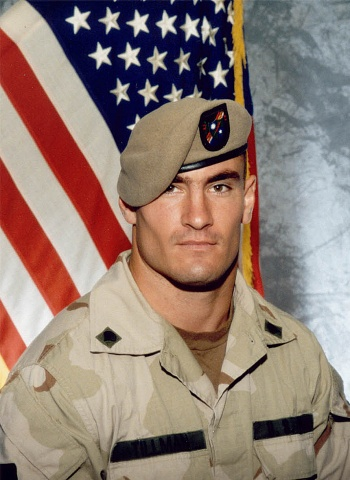
\includegraphics[width=1.75in]{./Images/Tillman.PNG}}
Pat Tillman, former Pac-10 Defensive Player of the Year and Arizona Cardinals safety, killed by friendly fire in Afghanistan in 2004.
\end{frame}

\begin{frame}{Less common?}
\centerline{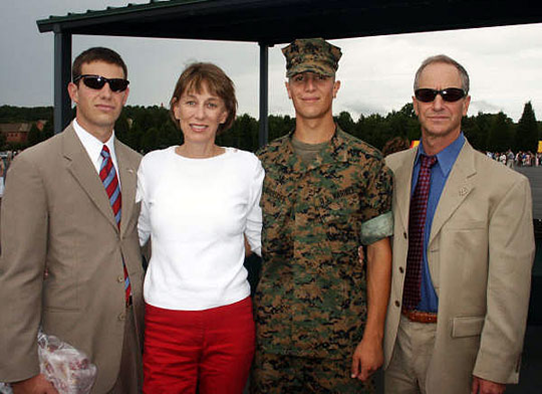
\includegraphics[width=3.25in]{./Images/Krissoff.PNG}}

Bill Krissoff, orthopedic surgeon, aged 61, enlisted in the Navy Medical Corps after his son Nathan was killed in the Marine Corps in Iraq in 2006.
\end{frame}



\section{Data}
\begin{frame}{\insertsectionhead}
\begin{itemize}
\item
FOIA: Recruits
\begin{itemize}
\item
Three separate sets of all Military Applicants, Contracts, Accessions from January 1990-July 2006.
\item
Active Duty (6.4m, 3.4m, 3.0m)
\item
Able to match 96\% to a ZIP
\end{itemize}

\item US military deaths
\begin{itemize}
 \item
 Public: Those considered to be part of OIF/OEF starting October 2001. (2886 before July '06)
 \item Able to match 94\% by county.
\item FOIA: Every death from January 1990-2010 (21,744)
\end{itemize}
\item Unemployment (BLS)
\item Mortality (NCHS--no geographic identifiers after 2004)
\item Quarterly Recruiters by State (through '04/'05)
\item FOIA: Military Occupational Specialty (MOS) 
\end{itemize}
\end{frame}

\begin{frame}{Data Acquisition}
How?
\begin{enumerate}
\item Spend too much time on Facebook
\item Realize you need more data
\item File FOIA request
\item ???
\item Profit!
\end{enumerate}
\end{frame}

\begin{frame}{Filing a FOIA Request}
Freedom of Information Act (1967)
\begin{itemize}
\item Right to information from government 
\item Nine exemptions \href{http://www.foiadvocates.com/exemptions.html}{\beamerbutton{Link}}
\begin{itemize}
\item National security
\item Personal privacy
\item Oil well information (of course)
\end{itemize}
\item File with relevant agency: DOD (\href{http://www.esd.whs.mil/FOID/Submit-Request/}{Broken link!})
\item Be specific!
\end{itemize}
\end{frame}

{ % all template changes are local to this group.
    \setbeamertemplate{navigation symbols}{}
    \begin{frame}[plain]
        \begin{tikzpicture}[remember picture,overlay]
            \node[at=(current page.center)] {
                \href{https://www.bitss.org/}{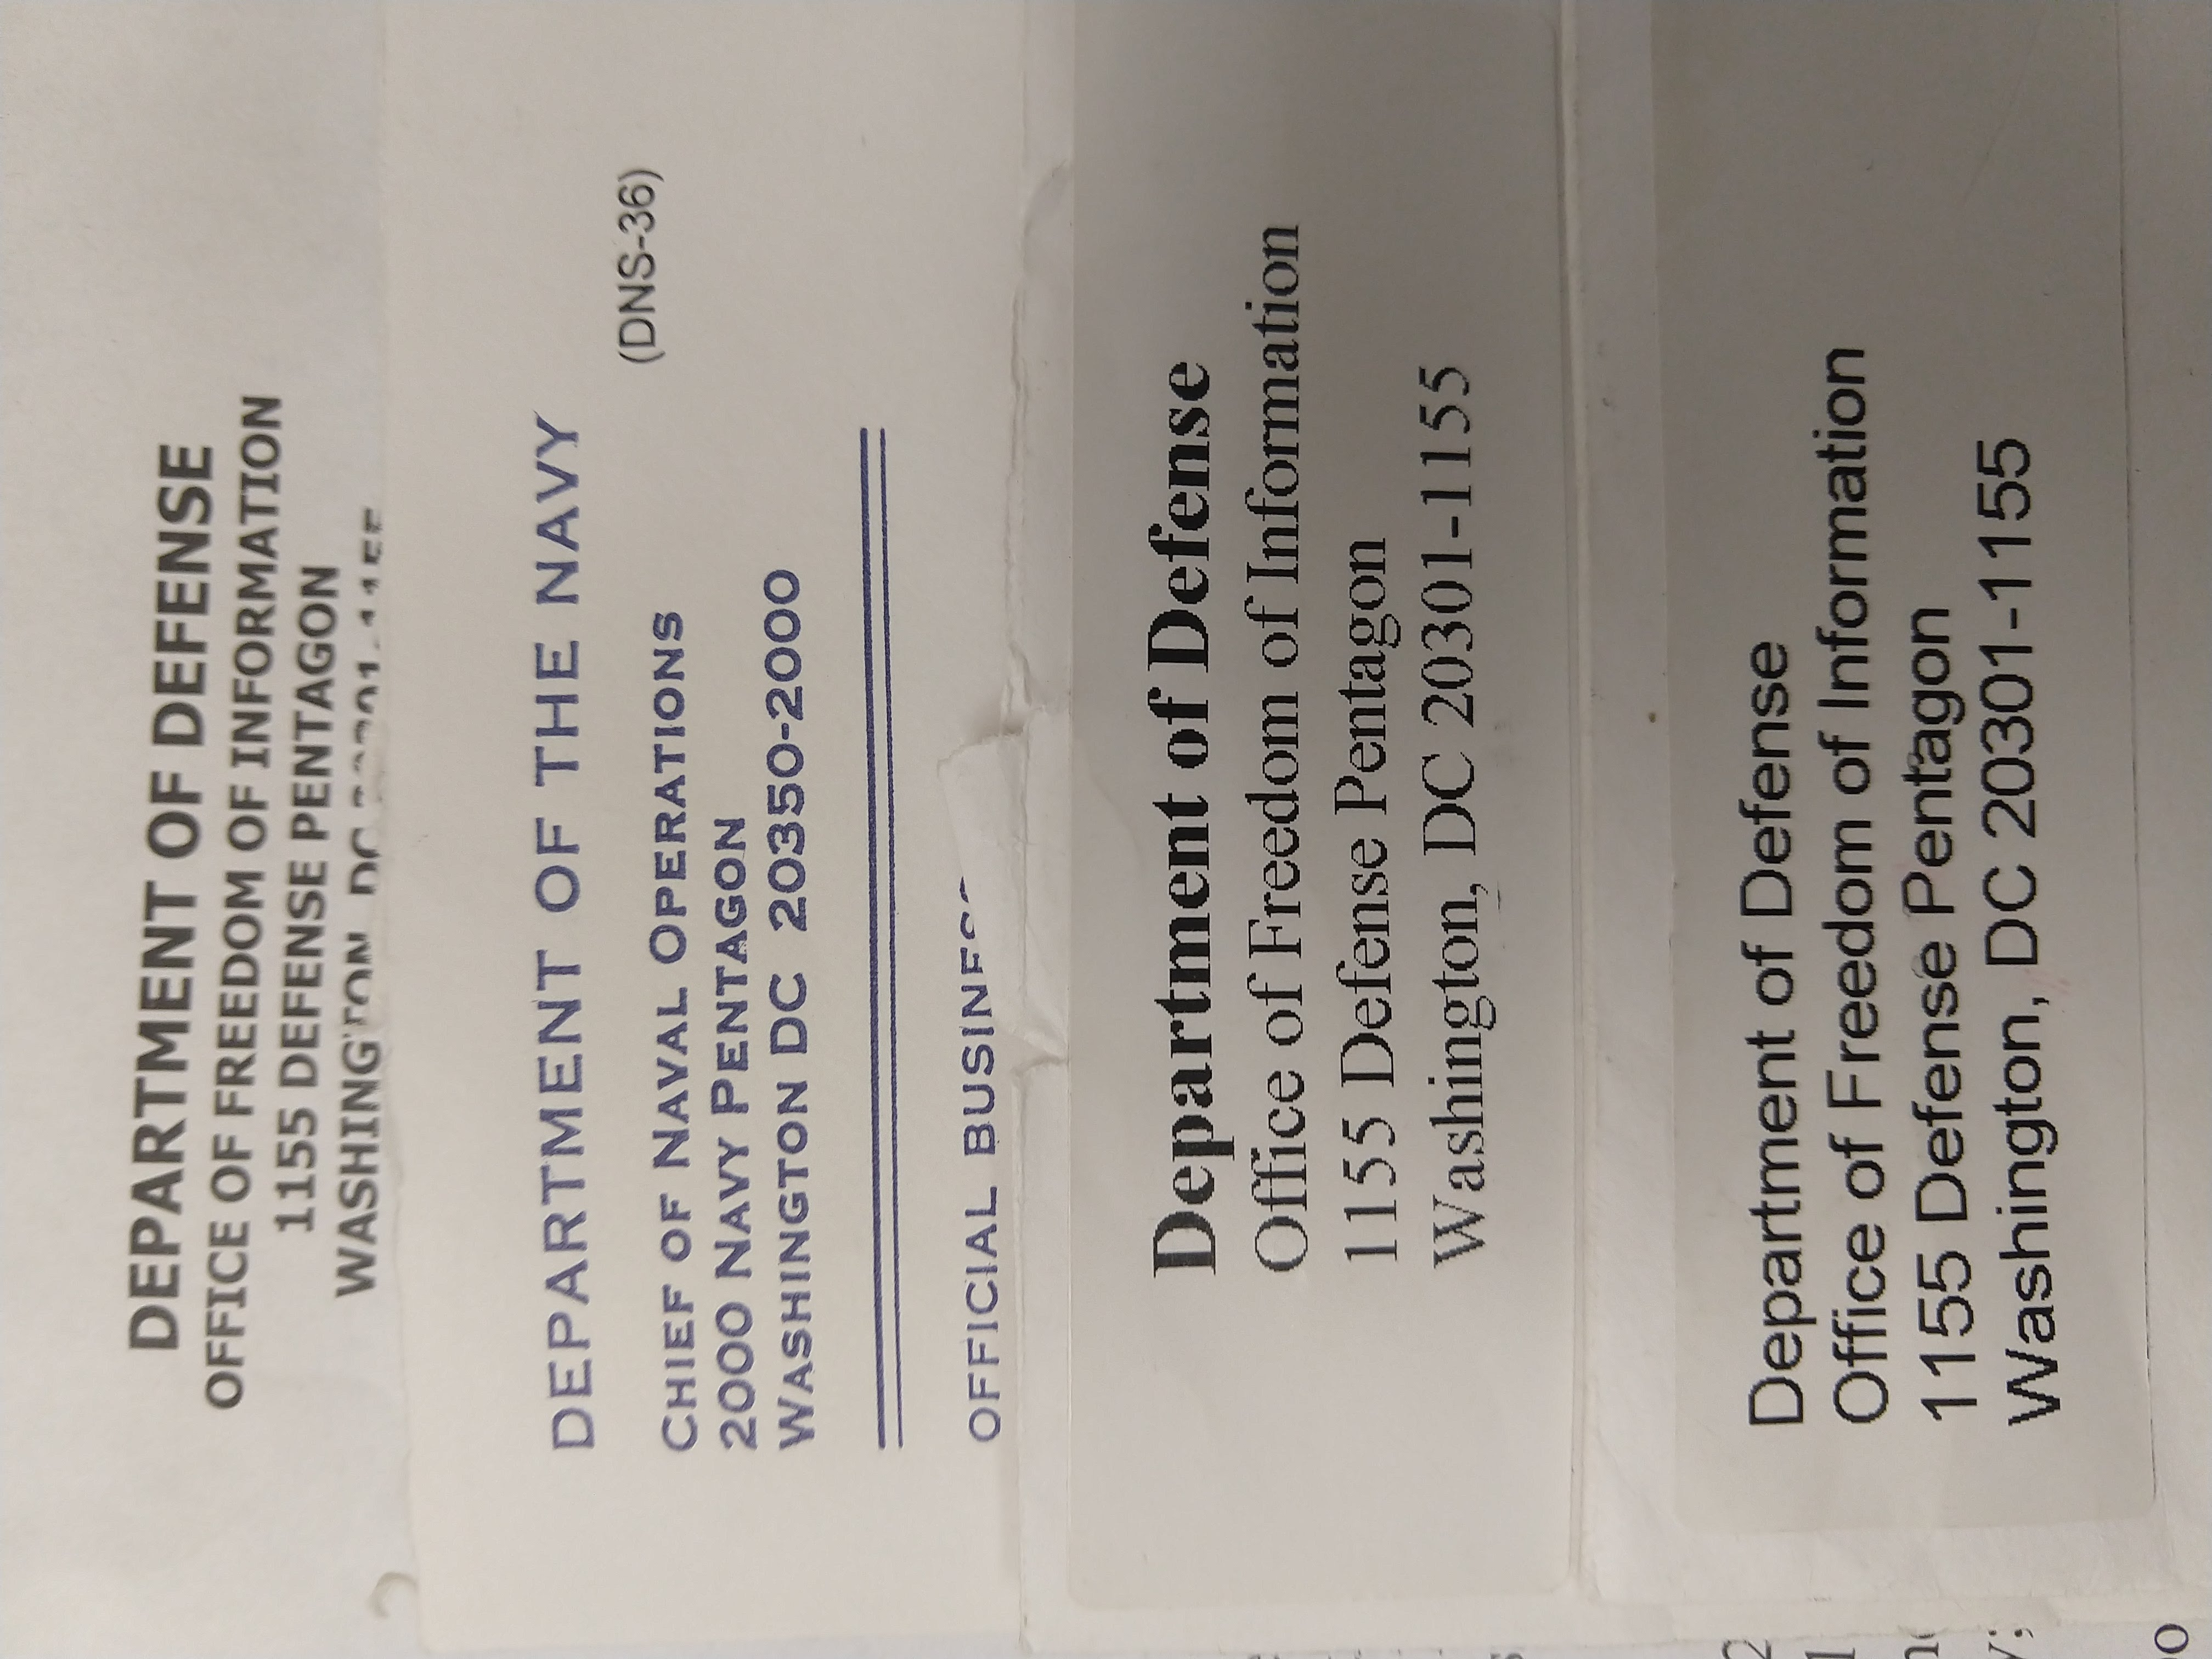
\includegraphics[height=3in, angle=270]{./Images/IMG_envelopes.jpg}}
            };
        \end{tikzpicture}
     \end{frame}
}


\begin{frame}[label=back]{Concerns}
\begin{itemize}
\item ``We will be unable to respond...'' \hyperlink{Moretime}{\beamerbutton{More}}
\item You'll never be able to run the SQL query yourself. Jump on mistakes fast!
\item Reduced/no fee for educational use? \hyperlink{More}{\beamerbutton{More}}
\end{itemize}
\end{frame}

\begin{frame}{Ask the Librarian!}
\centerline{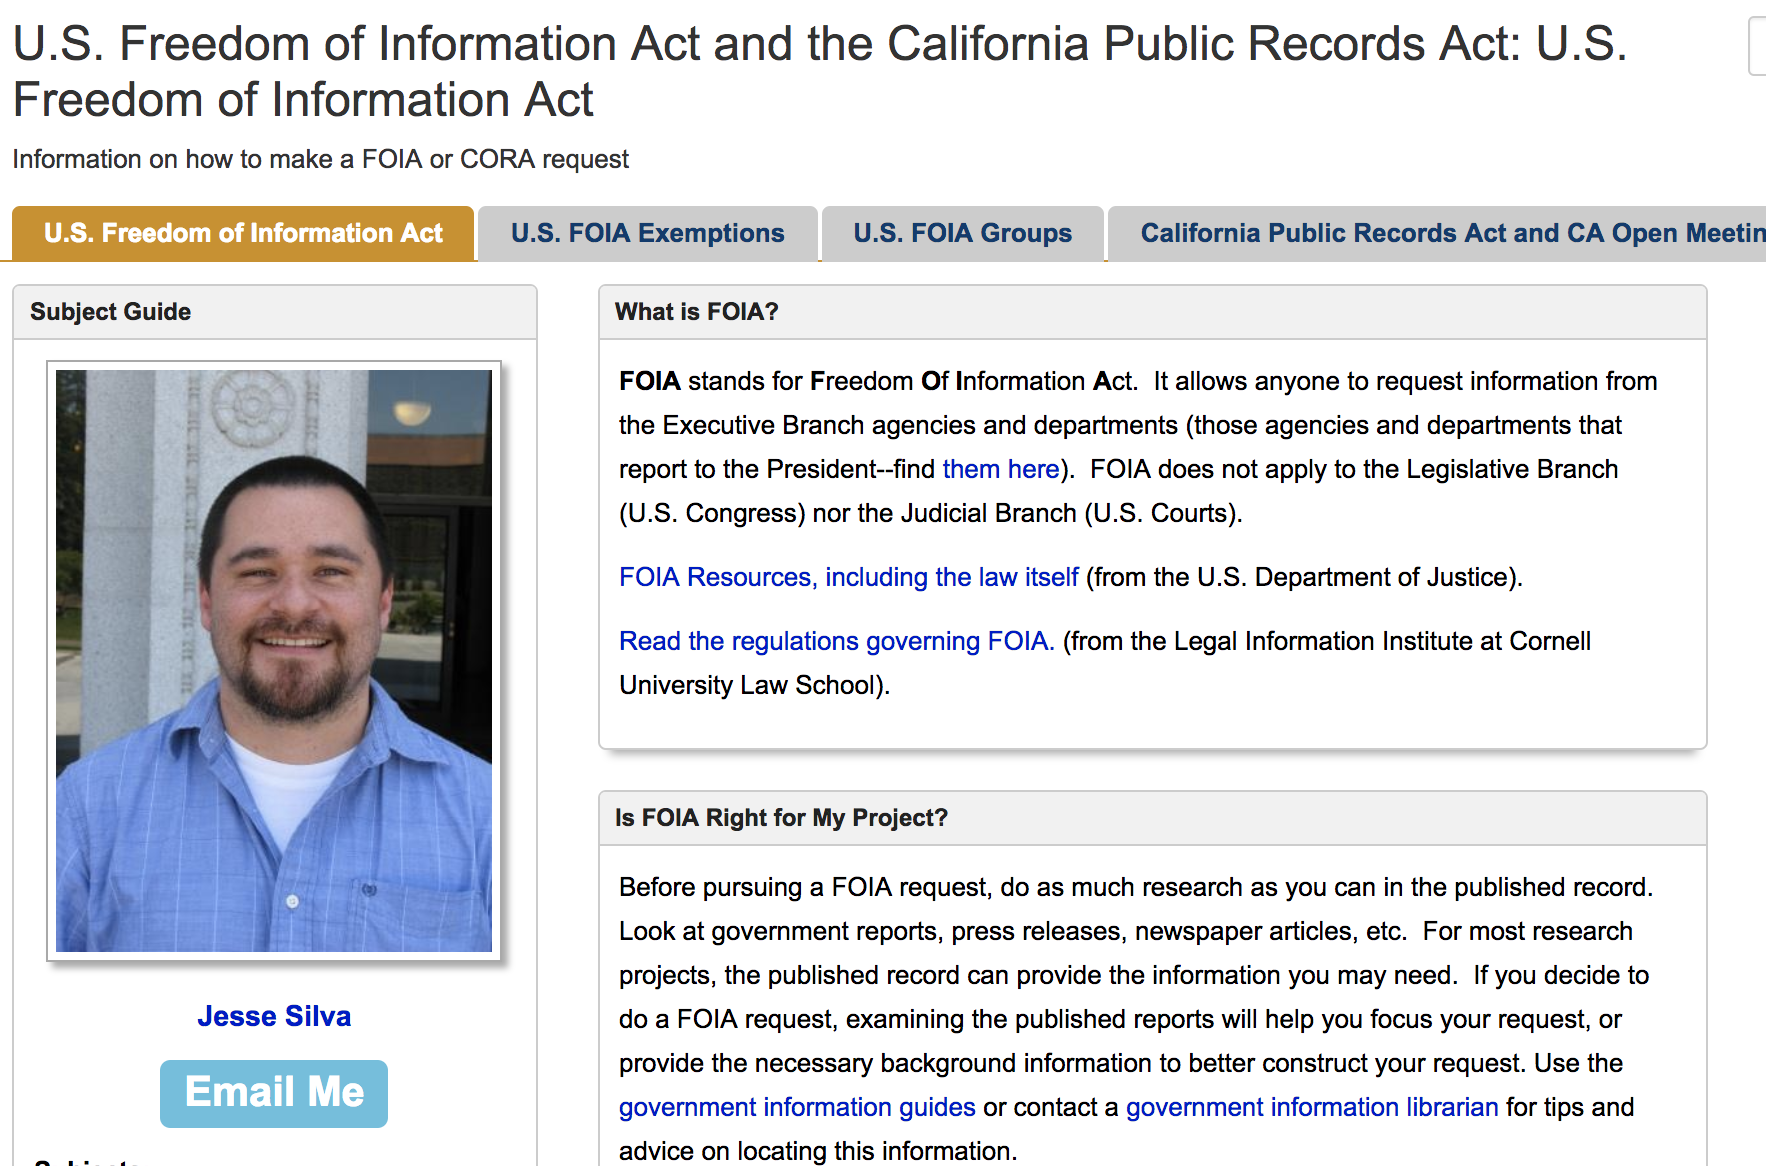
\includegraphics[width=4in]{./Images/Librarian.PNG}}
%Ask the librarian! \href{http://guides.lib.berkeley.edu/FOIA}{\beamerbutton{Link}}
\end{frame}

{ % all template changes are local to this group.
    \setbeamertemplate{navigation symbols}{}
    \begin{frame}[plain]
        \begin{tikzpicture}[remember picture,overlay]
            \node[at=(current page.center)] {
                \href{https://www.bitss.org/}{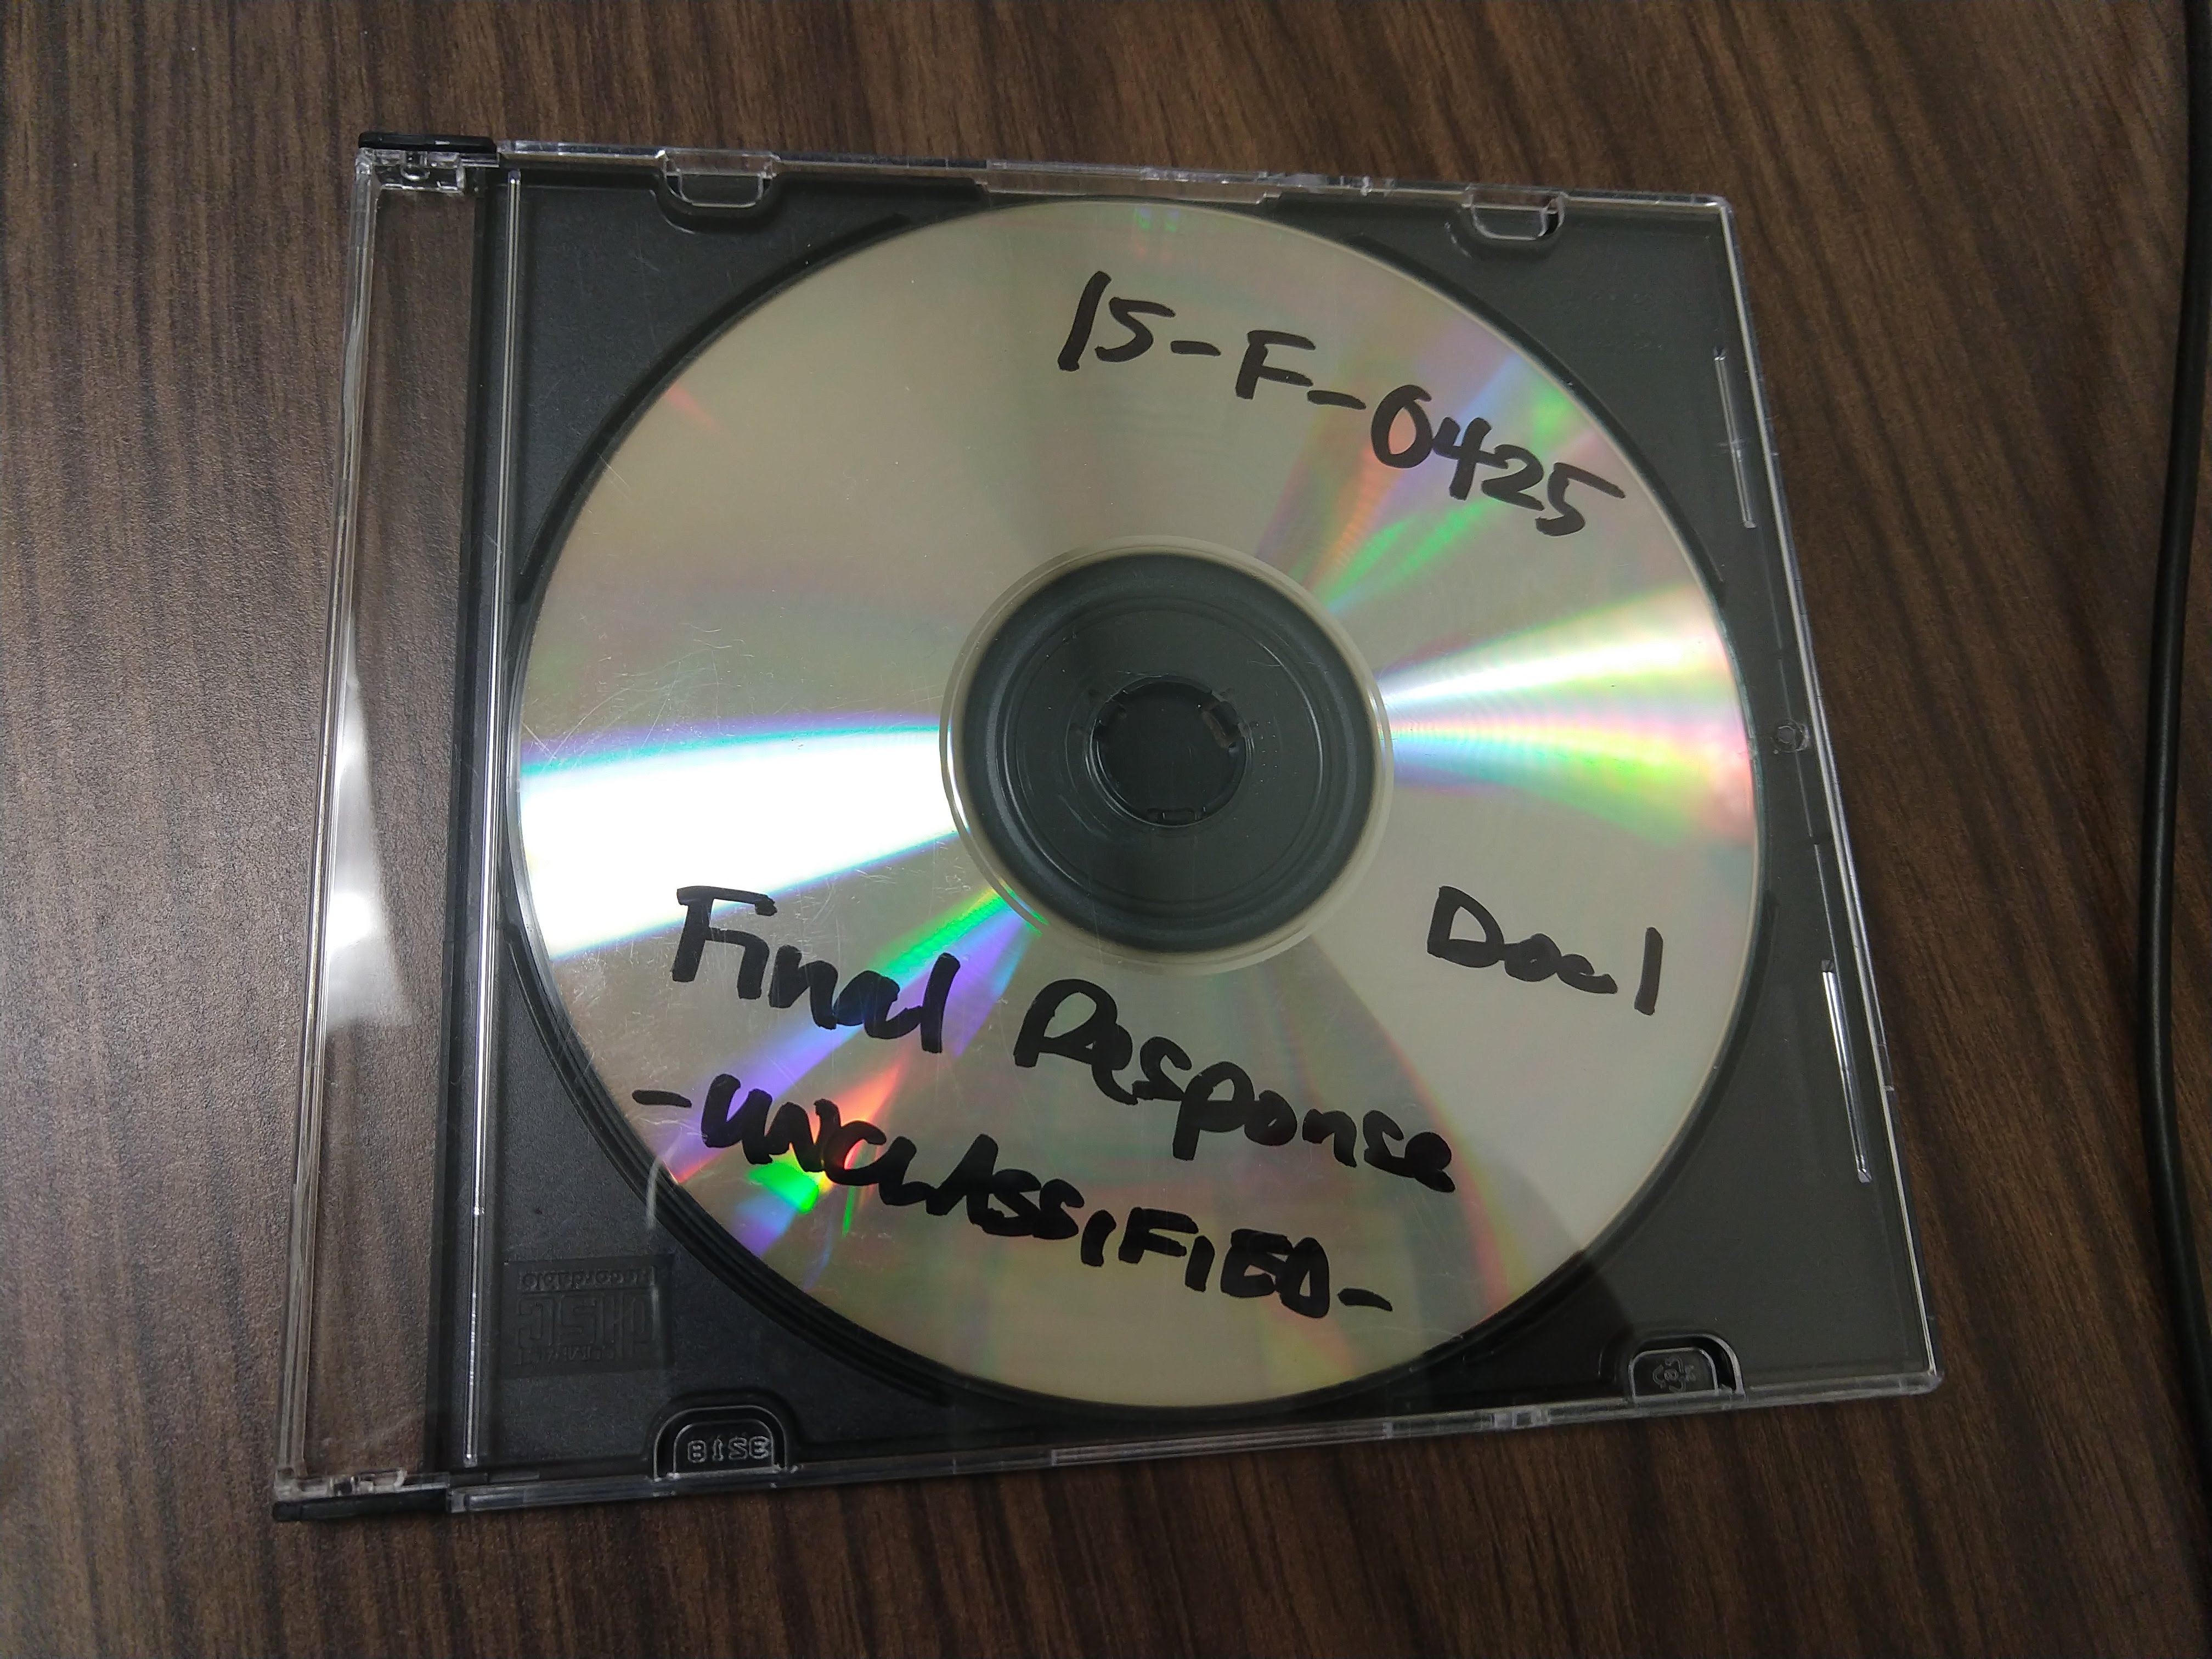
\includegraphics[height=\paperheight]{./Images/IMG_CD.jpg}}
            };
        \end{tikzpicture}
     \end{frame}
}

{ % all template changes are local to this group.
    \setbeamertemplate{navigation symbols}{}
    \begin{frame}[plain]
        \begin{tikzpicture}[remember picture,overlay]
            \node[at=(current page.center)] {
                \href{https://www.bitss.org/}{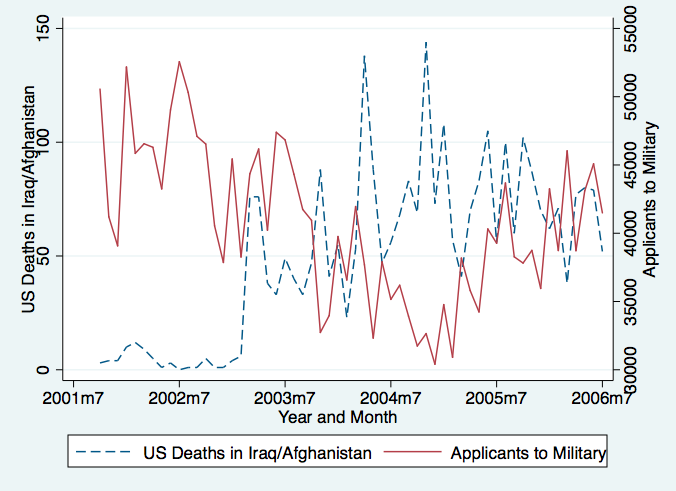
\includegraphics[height=\paperheight]{./Images/graph_deathsvsrecruits_basic.png}}
            };
        \end{tikzpicture}
     \end{frame}
}

{ % all template changes are local to this group.
    \setbeamertemplate{navigation symbols}{}
    \begin{frame}[plain]
        \begin{tikzpicture}[remember picture,overlay]
            \node[at=(current page.center)] {
                \href{https://www.bitss.org/}{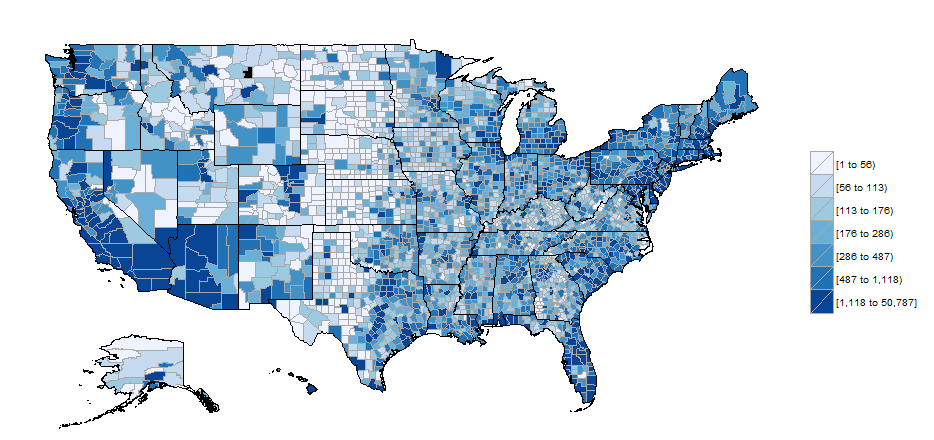
\includegraphics[width=\paperwidth]{./Images/recruits_rstudio.png}}
            };
        \end{tikzpicture}
     \end{frame}
}
{ % all template changes are local to this group.
    \setbeamertemplate{navigation symbols}{}
    \begin{frame}[plain]
        \begin{tikzpicture}[remember picture,overlay]
            \node[at=(current page.center)] {
                \href{https://www.bitss.org/}{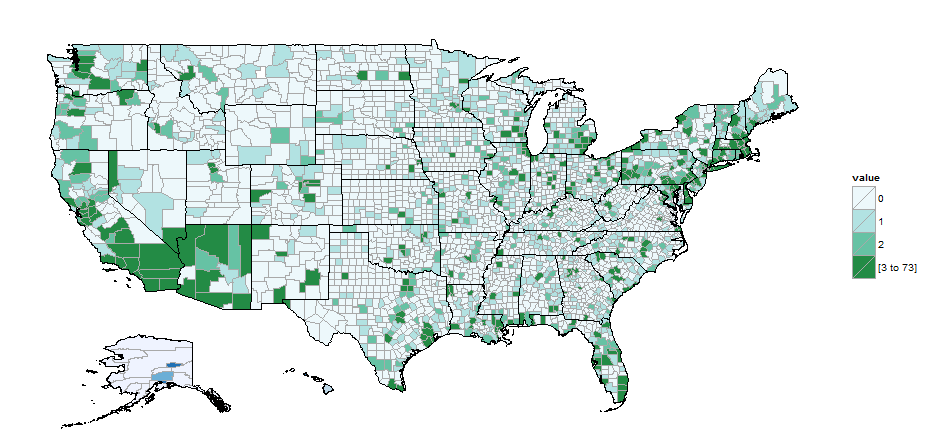
\includegraphics[width=\paperwidth]{./Images/deaths_rstudio.png}}
            };
        \end{tikzpicture}
     \end{frame}
}

{ % all template changes are local to this group.
    \setbeamertemplate{navigation symbols}{}
    \begin{frame}[plain]
        \begin{tikzpicture}[remember picture,overlay]
            \node[at=(current page.center)] {
                \href{https://www.bitss.org/}{
\includegraphics[height=\paperheight]{./Images/JEBOscreenshot.png}}
            };
        \end{tikzpicture}
     \end{frame}
}

\begin{frame}
\begin{center}
Questions?
\vspace{1in}


\Huge{Thank you!}
\end{center}
\end{frame}

\begin{frame}[label=Moretime]{More on Time}
 We will be unable to respond to your request within the FOIA's 20 day statutory time period as there are unusual circumstances which impact on our ability to quickly process your request.  These unusual circumstances are:  (a) the need to search for and collect records from a facility geographically separated from this Office and (b) the need for consultation with one or more other agencies or DoD components having a substantial interest in either the determination or the subject matter of the records.  For these reasons, your request has been placed in our complex processing queue and will be worked in the order the request was received.  Our current administrative workload is 1,633 open requests. \hyperlink{back}{\beamerbutton{Back}}
\end{frame}
 
\begin{frame}[label=More]{More on Cost}
\begin{small}
Per your request, you have set out that you are in the FOIA fee category of "Educational."  The intended use of the information you are seeking is not clear from the request itself, and we encourage you to give us additional information or clarification.  The school, UC Berkley, must show a use or purpose for the scholarly research.  As well, to qualify as an educational requester, your request has to be authorized by and made under the auspices of a qualifying institution that operates a program or programs of scholarly research that is not being accomplished for commercial use.  Scholarly research should further the goal of the institution, rather than an individual goal.  Please note that records requested for the intention of fulfilling credit requirements are not considered to be sought for a scholarly purpose; furthermore, students gathering data for research papers do not !
 qualify as educational requesters.

        Would you please provide some indication, on official school letterhead, that the information you are seeking is to be used by University of California, Berkley, prior to close of business, March 4, 2015.

        If I do not hear from you prior to that time, I will place your request in the "Other" fee category, vice the "Educational" fee category.  If you are placed in the "Other" fee category, you are entitled to the first two hours of search time at no charge, and the first 100 pages of duplication free of charge. Subsequent processing will be assessed at the established DoD fee rates of: professional search time, \$44 per hour; executive search time, \$75 per hour; and document reproduction at \$0.15 per page.

        Please note that the tasked component has provided a fee estimate totaling 48 hours of search/review at the professional rate of \$44 per hour, or a total cost estimate of approximately \$2,112.
        \hyperlink{back}{\beamerbutton{Back}}
        \end{small}
\end{frame}

\end{document}

